\documentclass{article}
\usepackage[a4paper,left=2.5cm,right=2.5cm,top=2.5cm,bottom=2.5cm]{geometry}
\usepackage[utf8]{inputenc}
\usepackage{titlesec}
\usepackage{hyperref}
\usepackage{enumitem}
\usepackage{graphicx}

\titleformat{\section}
{\normalfont\Large\bfseries}{Unit~\thesection}{1em}{}
\graphicspath{ {images/} }

\begin{document}

\begin{center}
	{\Large CIS*2520 Mock Exam (Summer 2017)} \\
	\smallskip
	All questions are available on Courselink via \url{https://courselink.uoguelph.ca/d2l/le/content/470592/Home}.
\end{center}

\medskip
\section{Lists, Stacks and Queues}

\begin{enumerate}
	\item Define the following with respect to software design:
		\begin{enumerate}[label=\alph*.]
			\item Modularity \\\\
			\item Reuse \\\\
			\item Maintainability \\\\
			\item Coupling \\\\
			\item Cohesion \\\\
		\end{enumerate}
	\item Define Test-Driven Development. \\\\
	\item List ten different programming languages as well as their level of abstraction (Moderate, High, Very High).
		\begin{enumerate}[label=\arabic*.]
			\item \rule{8cm}{0.1mm}
			\item \rule{8cm}{0.1mm}
			\item \rule{8cm}{0.1mm}
			\item \rule{8cm}{0.1mm}
			\item \rule{8cm}{0.1mm}
			\item \rule{8cm}{0.1mm}
			\item \rule{8cm}{0.1mm}
			\item \rule{8cm}{0.1mm}
			\item \rule{8cm}{0.1mm}
			\item \rule{8cm}{0.1mm} \\
		\end{enumerate}
	\item Write pseudocode for a multiply and a subtract operation for the fraction ADT. What does the integer portion of the Fraction struct represent? List any additional operation(s) that would be required in order to make use of that part of the struct. (Fraction ADT available on Courselink)
	\newpage
	\item Write the following three algorithms:
		\begin{enumerate}[label=\arabic*.]
			\item The algorithm for the addToLocation() operation for the List ADT. This operation should add an element to the list at a specific location in the list (identified by a number). Use the same specification format as has been used to describe operations in this lesson. Include all necessary parameters and return values in the signature of your specification. Be sure to include preconditions and postconditions.
			\vspace{3cm}
			\item The algorithm to delete a node from the nth position of a linked list. The operation should return the deleted data and ensure that the remaining elements of the list are properly connected.
			\vspace{3cm}
			\item The algorithm for inserting a node in sorted order given an array implementation of a list. The algorithm should take the data as a parameter.
			\vspace{3cm}
		\end{enumerate}
	\item Would a double linked list or a single linked list be a better choice for encapsulation in a Stack ADT? Justify your opinion.
		\vspace{3cm}
	\item Write the algorithms for push() and pop() given an array implementation of a stack. Show the stack struct definition as well.
		\vspace{4cm}
	\newpage
	\item Create a design or prototype of a reverse polish calculator program. You should limit operations to + - * and /. Use a stack ADT in your design.
	\newpage
	\item What is the Computation complexity of the enqueue() and dequeue() operations expressed in Big O notation? \\\\
	\item What additional information must be kept track of in order to use a conventional array as a circular buffer? Give the Queue struct that you would use if you were writing a circular buffer queue implementation.
	\vspace{4cm}
	\item Write the algorithm for dequeuing an item from a circular buffer queue.
	\vspace{4cm}
	\item Which of the following statements about queues is untrue?
		\begin{enumerate}[label=\alph*.]
			\item Queues can have elements inserted at any position in the data structure.
			\item The first element inserted into a queue will be the first element taken out of the queue.
			\item Queues can be found in the real world.
			\item The size of a queue data structure is bounded only by the size of the computer memory.
			\item A queue is somewhat similar to a stack.
		\end{enumerate}
	\item Which List operation would be most likely to be the one encapsulated if you were writing a remove operation for a queue?
		\begin{enumerate}[label=\alph*.]
			\item addHead(elementToBeAdded)
			\item length()
			\item removeBack()
			\item removeHead()
			\item insert(position, elementToBeAdded)
		\end{enumerate}
	\item Given the following queue: A B b E r S T, where A is the front of the queue, what will the queue content be after two remove operations?
		\begin{enumerate}[label=\alph*.]
			\item A B b E r S T
			\item b E r S T
			\item A B b E r S
			\item T A B b E r
			\item The queue will be empty.
		\end{enumerate}
	\newpage
	\item Given the following queue: t y 5 8 i 2 d t e, what should a call to length() return?
		\begin{enumerate}[label=\alph*.]
			\item 9
			\item 8
			\item 10
			\item It will generate an error because of the mixed data types.
			\item 3
		\end{enumerate}
\end{enumerate}

\medskip
\section{Hash Table and Binary Trees}

\begin{enumerate}
	\item If you were implementing a student record system for a small music school with fewer than 200 students, and were using associative arrays as the data structure, how would you implement your associative array? Would you make a different choice if your student record system was for a university?
	\vspace{2cm}
	\item Write a ’to-do list’ of the things you would need to do (including research and learning) in order to implement the borrowers’ library example. Try to make the list very specific. Use the to-do list to estimate the amount of time it would take you to implement and test the application (round up to the nearest hour).
	\vspace{5cm}
	\item Using the division method, calculate hash values for the following set of keys:
		\begin{center}	
			\(\{54, 77, 82, 13, 991, 308, 68, 45, 1001, 73\}\)
		\end{center}
		Calculate once using a table size of 11. Calculate a second time using a table size of 12. Do you notice anything about the distributions of the calculated values?
		\vspace{2cm}
	\newpage
	\item The expected search time for Linear probing can be calculated by the following formula:
		\begin{enumerate}[label=\roman*.]
			\item \(O(1 + {1 \over 1 - loadFactor})\) for a successful search.
			\item \(O(1 + {1 \over {(1 - loadFactor})^2})\) for an unsuccessful search.
		\end{enumerate}
		Create a chart showing the expected search times (successful and unsuccessful) for the following load factors: .10, .20., .30, .40, .50, .60, .70, .80, .85, .90, .95. \\
		What do these numbers tell you?
	\vspace{2cm}
	\item Suppose you have two hash functions H1 and H2 where H1(87) = 10, H2(87) = 3 and H1(42)=10, H2(42)=7. Further suppose that the key 87 is inserted into the table first and then the key of 42. Show the sequence of table positions tried when using random probing with a constant of 37 and a table size of 11.
	\vspace{4cm}
	\item The expected time for a search using Double hashing can be calculated by the following formula:
		\begin{enumerate}[label=\roman*.]
			\item \(O({1 \over loadFactor} \times (1 + ln({1 \over {1 - loadFactr}})))\) for a successful search.
			\item \(O({ 1 \over {1 - loadFactor}})\) for an unsuccessful search.
		\end{enumerate}
		Create a chart showing the expected search times (successful and unsuccessful) for the following load factors: .10, .20., .30, .40, .50, .60, .70, .80, .85, .90, .95. \\
		What do these numbers tell you?
	\vspace{2cm}
	\item The loadFactor of a hash table using separate chaining to resolve collisions is calculated as the number of \textbf{keys / the number of chains}. The expected length of search, successful or unsuccessful, of Separate Chaining is \(O(1 + loadFactor)\).
		\begin{enumerate}[label=\alph*.]
			\item Calculate a chart of the predicted search times for the following load factors: .10, .20., .30, .40, .50, .60, .70, .80, .85, .90, .95.
			\vspace{2cm}
			\item What do these numbers tell you?
			\newpage
			\item What factors would you consider when selecting a collision resolution approach for a hash table?
			\vspace{2cm}
		\end{enumerate}
	\item The order that nodes are inserted into a tree can greatly affect the structure of the tree. Draw the binary tree that is constructed by adding the seven names in the following order:
		\begin{enumerate}[label=\arabic*.]
			\item Sleepy
			\item Bashful
			\item Doc
			\item Dopey
			\item Sneezy
			\item Happy
			\item Grumpy
		\end{enumerate}
	\vspace{1.5cm}
	\item Trace the algorithms for level-order traversal using a hand drawn tree. What order are the nodes of the tree printed in? Can you tweak the algorithm to reverse the order?
	\vspace{6cm}
	\item One of the most frequent uses of a binary tree is as a search tree. The object is to search through the data to find out if a particular element is part of the data. Write a recursive find procedure for a binary tree. Start with the root node of the tree. Your procedure can be in \(C\) or in pseudocode. Be sure to pass in the compare function pointer.
	\vspace{6cm}
	\item Give the in-order traversal and the pre-order traversal of the tree shown below.
		\begin{center}
		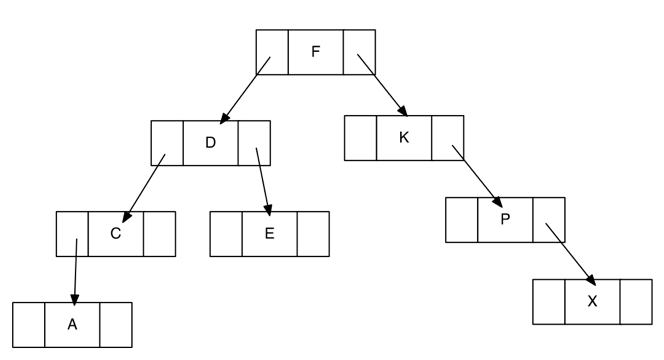
\includegraphics[scale=0.5]{tree}
		\end{center}
	\vspace{2cm}
	\item Write the pseudocode or \(C\) code for a compare operator. A compare operator must return three distinct values, one for when the first parameter is larger, one for when the second parameter is larger, and one for when the two parameters are equal. The convention is to use 1, 0, and -1 for the three values. Zero for equal values, 1 for the first string being larger, -1 for the second.
	\vspace{5cm}
	\item The delete operation relies on a recursive function to find the minimum value in a subtree. The minimum value will always be the leftmost leaf of the subtree. Write the findMinimum function (in pseudocode or in \(C\)).
	\vspace{5cm}
	\newpage
\end{enumerate}

\medskip
\section{Heaps and Priority Queues}

\medskip
\section{Balanced Trees and Sorting}

\end{document}
